\documentclass[11pt,a4paper]{article}

\usepackage[margin=2.4cm]{geometry}
\usepackage{amsmath,amssymb}
\usepackage{booktabs}
\usepackage{array}
\usepackage{xcolor}
\usepackage{enumitem}
\usepackage{parskip}
\usepackage{microtype}
\usepackage{listings}
\usepackage{graphicx}
\usepackage[font=small,labelfont=bf]{caption}
\usepackage[colorlinks=true,linkcolor=blue!60!black,urlcolor=blue!60!black,citecolor=blue!60!black]{hyperref}
\graphicspath{{diagrams/}{../fno_t4_full/fno/}}

\definecolor{accent}{RGB}{42,120,214}
\definecolor{codebg}{RGB}{247,247,245}
\definecolor{inkgray}{RGB}{82,81,78}

\lstset{
  basicstyle=\ttfamily\small,
  backgroundcolor=\color{codebg},
  frame=single,
  framerule=0pt,
  xleftmargin=6pt,
  xrightmargin=6pt,
  breaklines=true,
  columns=fullflexible,
  keepspaces=true,
}

\newcommand{\intuition}[1]{\par\smallskip\noindent\textit{\color{inkgray}Intuition: #1}\par\smallskip}

\title{\textbf{Neural PDE Solvers for the 1D Elastic Wave Equation}\\[4pt]
\large Technical Reference: Problem Setup, PINN Arm, and the Fourier Neural Operator Baselines}
\author{SciML Project --- Ayush Debnath}
\date{July 2026}

\begin{document}
\maketitle
\tableofcontents
\newpage

%=====================================================================
\section{The Physical Problem}
%=====================================================================

The project solves the one-dimensional elastic wave equation in \emph{conservative form}:
\begin{equation}
  \rho(x)\, u_{tt} \;=\; \partial_x\!\bigl[\,E(x)\, u_x\,\bigr],
  \qquad x \in [x_{\min}, x_{\max}],\; t \in [0, 1],
  \label{eq:pde}
\end{equation}
where $u(x,t)$ is displacement, $E(x)$ the stiffness profile, and $\rho(x)$ the density.
The local wave speed is $c(x) = \sqrt{E(x)/\rho(x)}$.

The conservative form matters. Expanding the flux term gives
$E(x)\,u_{xx} + E'(x)\,u_x$; the naive reduction $u_{tt} = c^2 u_{xx}$
silently drops the $E'(x)\,u_x$ term and therefore gets reflection and
transmission at material interfaces wrong. Every solver in the repository
(finite differences, PINN losses, FNO training data) uses the conservative form.

\intuition{a wave hitting a stiffness jump partially bounces back and partially
passes through. The dropped term is exactly the part of the physics that
encodes this splitting.}

%=====================================================================
\section{Nondimensionalization}
%=====================================================================

All computation happens in nondimensional units, defined per material
(\texttt{wave/materials.py}, class \texttt{MaterialModel}). Given the physical
domain $[x^{\mathrm{phys}}_{\min}, x^{\mathrm{phys}}_{\max}]$ and reference
constants $E_{\mathrm{ref}}, \rho_{\mathrm{ref}}$:
\begin{align}
  L_{\mathrm{ref}} &= \tfrac{1}{2}\bigl(x^{\mathrm{phys}}_{\max}-x^{\mathrm{phys}}_{\min}\bigr), &
  V_{\mathrm{ref}} &= \sqrt{E_{\mathrm{ref}}/\rho_{\mathrm{ref}}}, &
  T_{\mathrm{ref}} &= L_{\mathrm{ref}} / V_{\mathrm{ref}},
\end{align}
so that $x \in [-1, 1]$, wave speeds are $O(1)$, and all PDE coefficients are
order one. Conversions back to physical units are
$x^{\mathrm{phys}} = x\,L_{\mathrm{ref}}$, $t^{\mathrm{phys}} = t\,T_{\mathrm{ref}}$,
and the source width scales as $\sigma_g = \sigma_g^{\mathrm{phys}} / L_{\mathrm{ref}}$.

\intuition{neural networks train badly when inputs and coefficients span wildly
different scales (stiffness in the tens vs.\ coordinates in $[-1,1]$).
Nondimensionalizing is one of the standard ``make PINNs actually work'' steps.}

%=====================================================================
\section{Material Models}
%=====================================================================

Three canonical materials of increasing difficulty (\texttt{wave/materials.py});
density is $\rho \equiv 1$ in all of them, so only stiffness varies and
$c(x) = \sqrt{E(x)}$.

\begin{center}
\begin{tabular}{@{}llll@{}}
\toprule
Model & Physical domain & $E_{\mathrm{ref}}$ & Stiffness profile (nondim.) \\
\midrule
\texttt{Homogeneous} & $[-1,1]$   & 80 & $E = 1$ everywhere \\
\texttt{TwoLayer}    & $[-1,1]$   & 80 & $1.0 \to 1.5$ jump at $x=0$ \\
\texttt{MultiLayer}  & $[-1.5,1.5]$ & 60 & 6 layers, $1.0 \to 2.5$ staircase \\
\bottomrule
\end{tabular}
\end{center}

\paragraph{Smoothed interfaces.}
Material jumps are represented by a differentiable $\tanh$ switch rather than a
true discontinuity. For a single interface at $x_b$ with transition width
$w = 0.02/L_{\mathrm{ref}}$:
\begin{equation}
  \alpha(x) = \tfrac{1}{2}\Bigl(1 + \tanh\tfrac{x - x_b}{w}\Bigr), \qquad
  E(x) = E_L\,(1-\alpha) + E_R\,\alpha .
  \label{eq:tanh}
\end{equation}
$\alpha$ runs smoothly from 0 (left material) to 1 (right material) over a
width of a few $w$. The \texttt{MultiLayer} model chains this blend across its
five interfaces (at $x = -\tfrac{2}{3}, -\tfrac{1}{3}, 0, \tfrac{1}{3}, \tfrac{2}{3}$
in nondimensional units, values $E \in \{1.0, 1.3, 1.6, 1.9, 2.2, 2.5\}$).
Because interfaces are $\sim 0.33$ apart while transitions are $\sim 0.013$
wide, each blend reduces locally to a clean two-value crossfade.

\intuition{the PINN loss needs $\partial_x[E\,u_x]$, so $E(x)$ must be
differentiable --- a step function has no usable gradient. The FD solver instead
handles jumps with harmonic averaging (Section~\ref{sec:fd}); two different
answers to the same problem.}

\begin{figure}[htb]
  \centering
  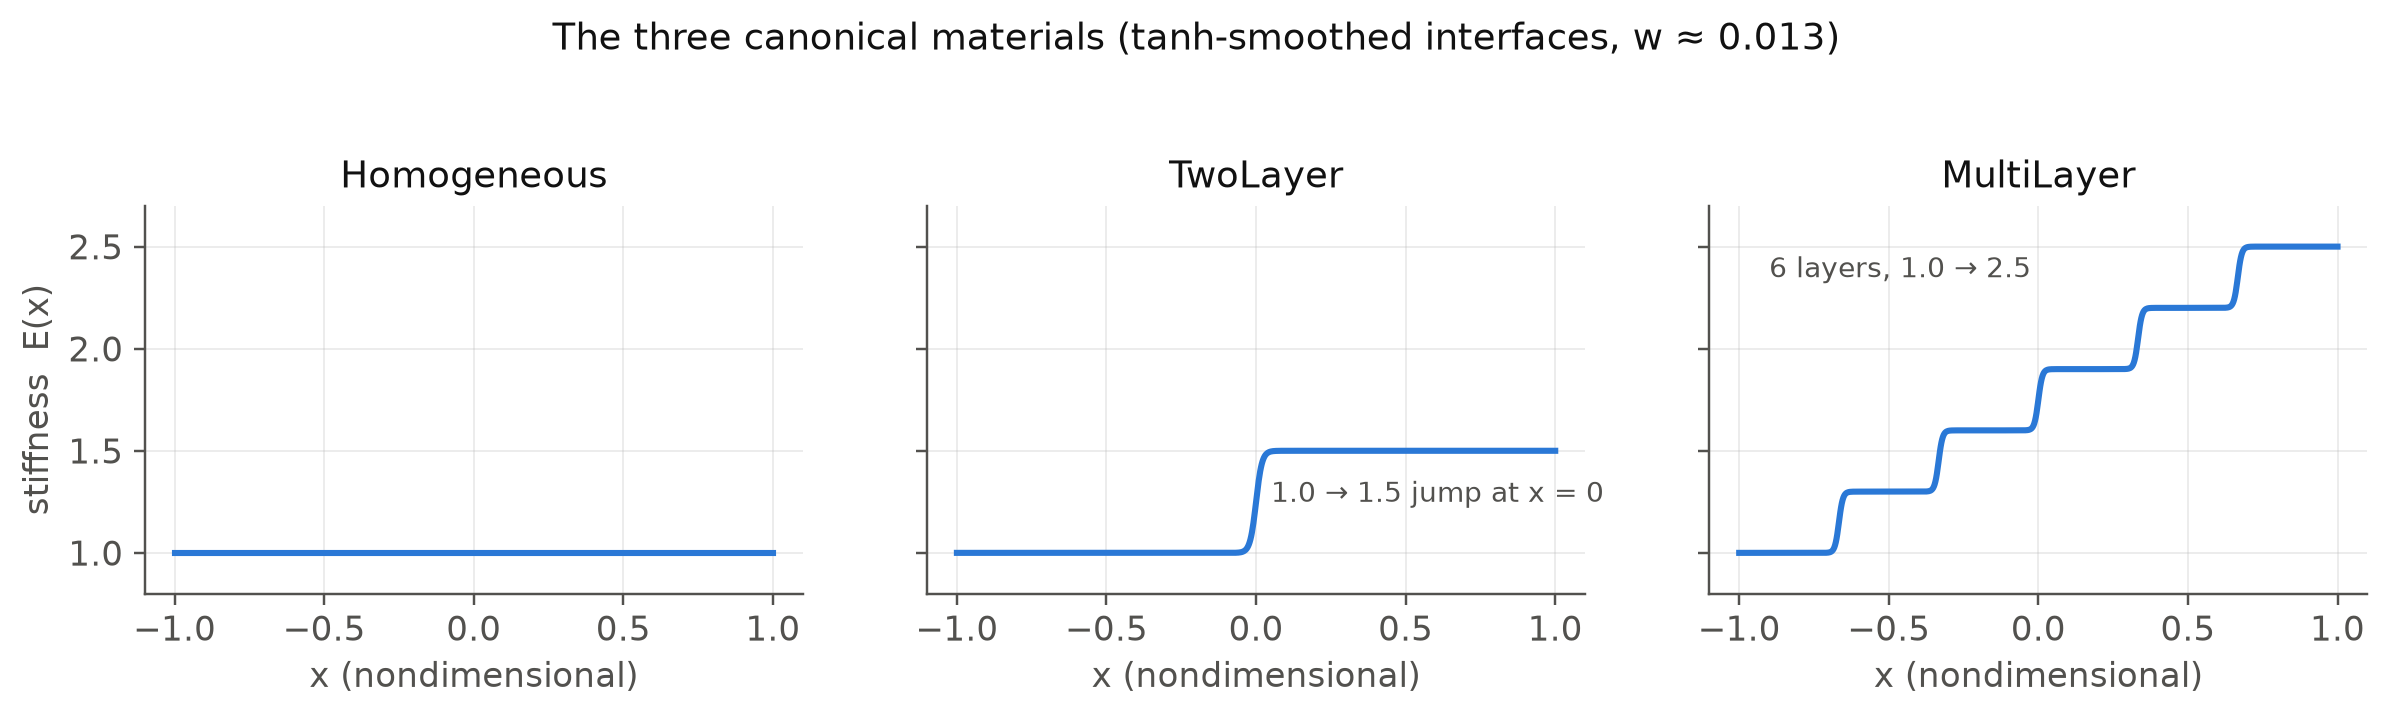
\includegraphics[width=\linewidth]{plot_materials.png}
  \caption{Stiffness profiles $E(x)$ of the three canonical materials.
  All interfaces are tanh-smoothed with width $w\approx 0.013$.}
  \label{fig:materials}
\end{figure}

%=====================================================================
\section{Initial Condition and the Hard-Constraint Ansatz}
\label{sec:ansatz}
%=====================================================================

\paragraph{Initial displacement.} A normalized first derivative of a Gaussian
(\texttt{gaussian\_ic} in \texttt{wave/problem\_data.py}), an antisymmetric
single-wiggle pulse of width $\sigma_g = 0.1$ centred at $x_0 = 0$:
\begin{equation}
  f(x) = \exp\!\Bigl(-\tfrac{(x-x_0)^2}{2\sigma_g^2}\Bigr), \qquad
  g(x) = \frac{f'(x)}{\max_x |f'(x)|},
  \qquad u(x,0) = g(x),\; u_t(x,0) = 0 .
\end{equation}
The normalization makes the peak amplitude exactly 1 (raw $|f'|$ peaks at
$(1/\sigma_g)\,e^{-1/2} \approx 6.07$ at $x = x_0 \pm \sigma_g$).

\paragraph{The ansatz.} Instead of penalizing initial-condition errors, the
solution is \emph{assumed to have the form}
\begin{equation}
  \hat{u}(x,t) \;=\;
  \underbrace{g(x)\, e^{-\frac{1}{2}(15t)^2}}_{\text{known IC, fading out}}
  \;+\;
  \underbrace{\tanh^2(25t)}_{\text{gate}} \cdot
  \underbrace{N_\theta(x,t)}_{\text{learned ``NN term''}} .
  \label{eq:ansatz}
\end{equation}
Both initial conditions hold \emph{exactly, by construction}:
\begin{itemize}[nosep]
  \item At $t=0$: the exponential equals 1 and $\tanh^2(0)=0$, so
        $\hat{u}(x,0) = g(x)$ regardless of the network output.
  \item For velocity: $\frac{d}{dt}e^{-\frac{1}{2}(15t)^2} = -225\,t\,e^{(\cdot)} \to 0$
        and $\frac{d}{dt}\tanh^2(25t) = 50\tanh(25t)\operatorname{sech}^2(25t) \to 0$
        at $t=0$ (the \emph{squaring} of the tanh is what kills the slope), so
        $\hat{u}_t(x,0) = 0$ exactly.
\end{itemize}
The constants 15 and 25 set the handoff window: the IC term is negligible by
$t \approx 0.2$ and the gate is fully open by $t \approx 0.1$. The network
therefore owns $\sim 90\%$ of the time domain, and the optimizer never has to
fight for the initial condition. All derivatives in the PDE residual are taken
through the \emph{assembled} $\hat u$, not the raw network.

\begin{figure}[htb]
  \centering
  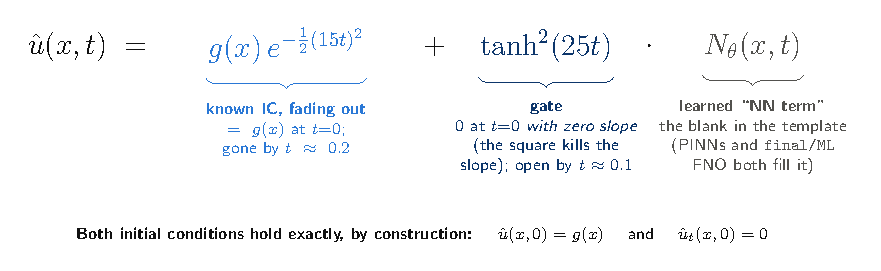
\includegraphics[width=0.85\linewidth]{diag_ansatz_anatomy.pdf}
  \caption{Anatomy of the hard-constraint ansatz: the template owns $t=0$,
  the network owns everything after.}
  \label{fig:ansatz}
\end{figure}

\begin{figure}[htb]
  \centering
  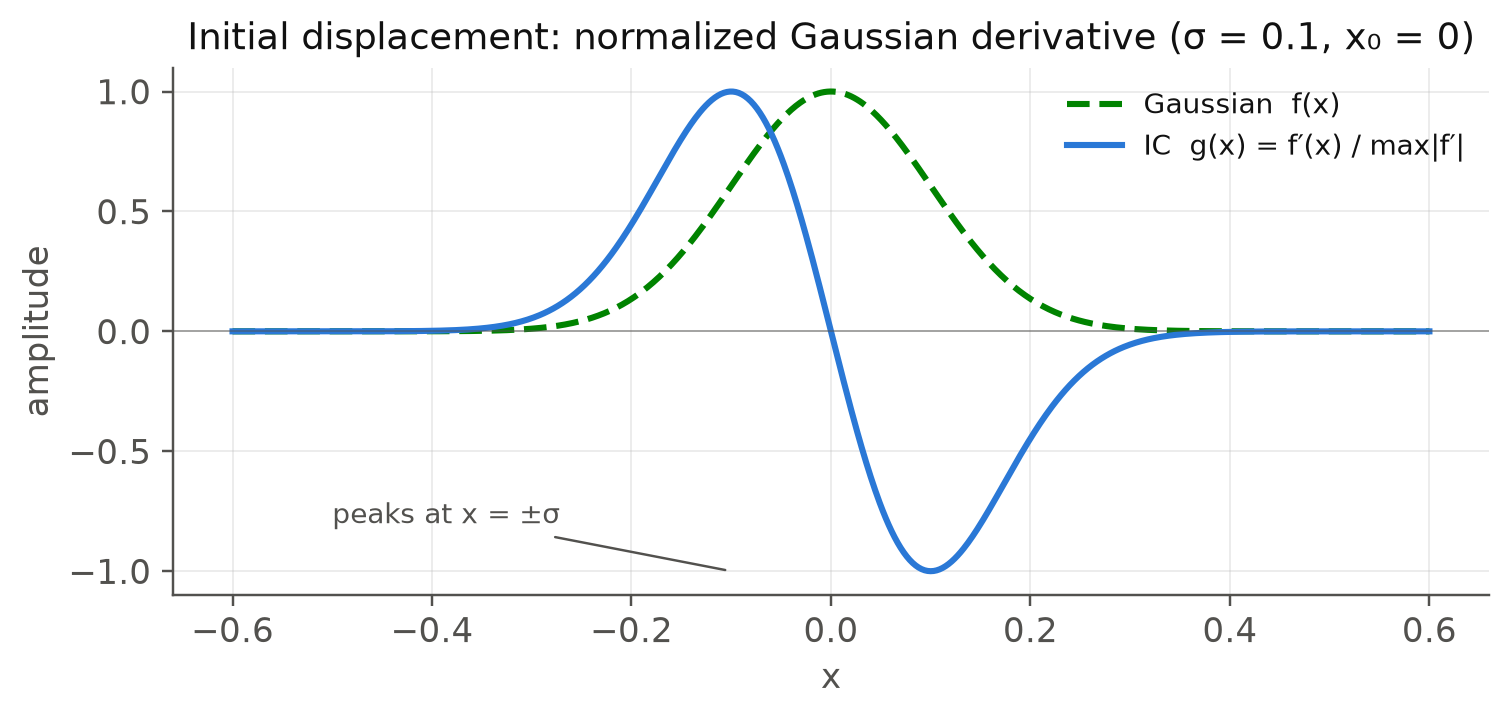
\includegraphics[width=0.48\linewidth]{plot_gaussian_ic.png}\hfill
  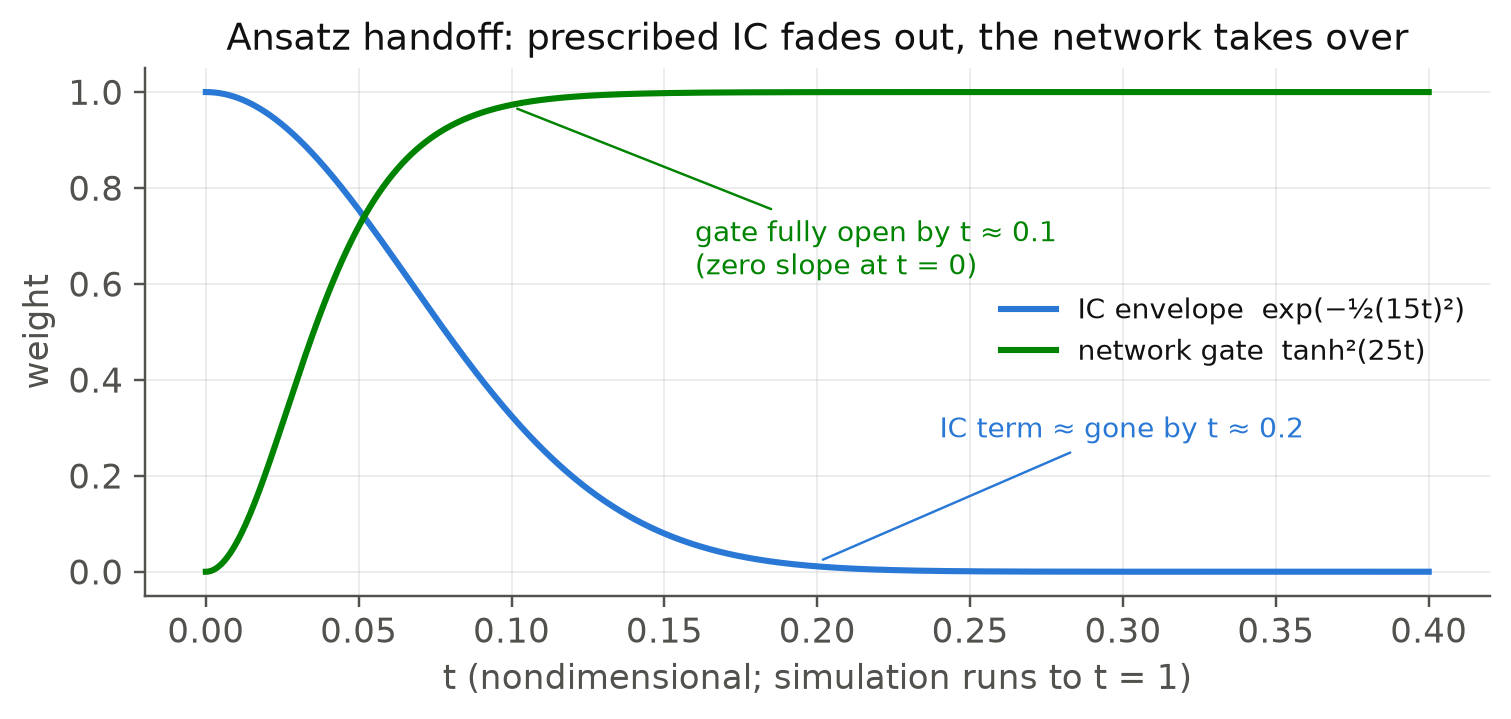
\includegraphics[width=0.48\linewidth]{plot_ansatz_gates.png}
  \caption{Left: the initial pulse $g(x)$ (normalized Gaussian derivative)
  and its parent Gaussian. Right: the two time gates of the ansatz --- the
  prescribed IC fades out while the network gate opens.}
  \label{fig:gates}
\end{figure}

\intuition{an ansatz is a fill-in-the-blanks template: ``the solution starts as
this exact pulse, fades that in and out smoothly, and here is a blank for
whatever happens afterwards.'' The network learns only the blank ---
the \emph{NN term}. Its raw output looks nothing like the wave; it is the
correction the template still needs.}

%=====================================================================
\section{The Finite-Difference Reference Solver}
\label{sec:fd}
%=====================================================================

\texttt{wave/fd\_solver.py} provides ground truth for everything: PINN scoring,
FNO training labels, and FNO evaluation. It integrates \eqref{eq:pde} with an
explicit second-order leapfrog scheme in flux form. With
$\lambda_i = \Delta t^2 / (\rho_i\,\Delta x^2)$:
\begin{equation}
  u_i^{n+1} = 2u_i^n - u_i^{n-1}
  + \lambda_i \Bigl[ E_{i+\frac12}\,(u_{i+1}^n - u_i^n) - E_{i-\frac12}\,(u_i^n - u_{i-1}^n) \Bigr],
\end{equation}
with \emph{harmonic-mean} interface stiffness
\begin{equation}
  E_{i+\frac12} = \frac{2\,E_i\,E_{i+1}}{E_i + E_{i+1}},
\end{equation}
which preserves correct transmission/reflection behaviour across interfaces.
The first step uses a Taylor start
$u_i^1 = u_i^0 + \Delta t\, g_i + \tfrac12 \lambda_i\,[\text{flux}]_i^0$.

\paragraph{Stability.} The time step obeys the CFL condition
$\Delta t = \mathrm{CFL} \cdot \Delta x / \max_x c(x)$ with safety factor
$\mathrm{CFL} = 0.9$; the solver picks its own $\Delta t$ and callers
re-interpolate onto their target time grid.

\paragraph{Absorbing boundaries.} First-order radiation conditions
$u_t \mp c\,u_x = 0$ discretized with the \emph{Mur} scheme,
\begin{equation}
  u_0^{n+1} = u_1^{n} + \beta\,(u_1^{n+1} - u_0^{n}), \qquad
  \beta = \frac{c\,\Delta t - \Delta x}{c\,\Delta t + \Delta x},
\end{equation}
mirrored on the right boundary. (The seemingly natural centred-time /
one-sided-space discretization is unconditionally unstable.)

\paragraph{Why FD as the teacher.} No closed-form solution exists for layered
media; FD is provably convergent with understood error and stability; it is the
\emph{single} referee for all arms of the project, keeping rankings meaningful;
and in 1D it is cheap enough to run hundreds of times. (In 3D the economics
flip --- which is precisely when operator learning starts to pay.)

%=====================================================================
\section{The PINN Arm in Brief}
%=====================================================================

Seven architectures share the identical ansatz \eqref{eq:ansatz}, losses, and
two-phase training (Adam $\to$ L-BFGS):

\begin{center}
\begin{tabular}{@{}ll@{}}
\toprule
Architecture & Key idea \\
\midrule
\texttt{VanillaPINN}       & MLP, tanh activations, Xavier init \\
\texttt{FourierFeaturePINN}& trainable random Fourier embedding $\to$ MLP \\
\texttt{PirateNet}         & fixed Fourier embed, RWF layers, residual blocks ($\alpha{=}0$ init) \\
\texttt{WavKAN}            & wavelet-based Kolmogorov--Arnold network \\
\texttt{KAN} (pykan)       & spline-based KAN \\
\texttt{ChebyshevKAN}      & Chebyshev-recurrence edges (cPIKAN) \\
\texttt{FourierWavKAN}     & Fourier embedding $\to$ WavKAN trunk \\
\bottomrule
\end{tabular}
\end{center}

Training machinery (\texttt{src/losses/wave\_loss.py}), summarized:
\begin{itemize}[nosep]
  \item \textbf{Causal weighting} (Wang et al.\ 2022): time split into 16 slabs;
        slab $m$ weighted by $w_m = \exp\bigl(-\varepsilon \sum_{k<m} L_k\bigr)$
        so late times only count once early times are solved.
  \item \textbf{GradNorm} (Wang et al.\ 2023): EMA-smoothed gradient-norm
        balancing of $w_{\mathrm{pde}}, w_{\mathrm{bc}}, w_{\mathrm{ic}}$, updated every 100 steps.
  \item \textbf{RBA}: pointwise residual-based attention
        $\lambda \leftarrow 0.999\lambda + 0.01\,|r|/\max|r|$, loss $=\overline{(\lambda r)^2}$.
  \item \textbf{SOAP}: Adam in the Shampoo eigenbasis (2D parameters only).
  \item \textbf{Absorbing BCs} as loss terms; checkpoint selection by a
        stationary validation metric; L-BFGS runs with causal weighting off.
\end{itemize}

The essential property for what follows: \emph{a PINN is trained per material},
taking hours per case, with elaborate machinery required to make the physics
loss optimizable at all.

%=====================================================================
\section{Why Operator Learning}
%=====================================================================

A PINN answers one question: ``what is $u(x,t)$ for \emph{this} material and
\emph{this} pulse?'' The Fourier Neural Operator (FNO; Li et al.\ 2020) instead
learns the \emph{map}
\begin{equation}
  \mathcal{G}: \bigl(E(x),\, \rho(x),\, g(x)\bigr) \;\longmapsto\; u(x,t),
\end{equation}
so a \emph{new} material costs one forward pass ($\sim$milliseconds) instead of
a fresh optimization ($\sim$hours). The trade: the FNO needs a solver-generated
dataset and inherits its training distribution and grid.

\begin{center}
\begin{tabular}{@{}p{4.4cm}p{4.6cm}p{4.6cm}@{}}
\toprule
 & Coordinate solver (PINN) & Neural operator (FNO) \\
\midrule
Learns & $(x,t) \mapsto u$, one case & material $\mapsto$ wavefield, a family \\
Supervision & PDE + BC + IC losses & FD solutions (plain regression) \\
New material & retrain from scratch & one forward pass \\
Data required & none & 768 FD solves \\
Mesh & mesh-free & grid-to-grid \\
Training difficulty & high (causal, GradNorm, \dots) & low (MSE + AdamW) \\
\bottomrule
\end{tabular}
\end{center}

\begin{figure}[htb]
  \centering
  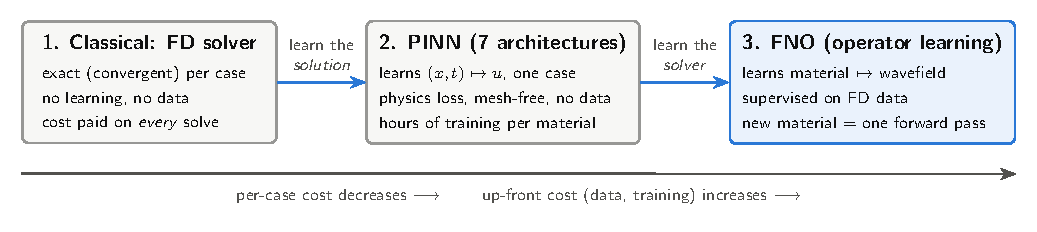
\includegraphics[width=\linewidth]{diag_evolution.pdf}
  \caption{The three solver paradigms in the project, ordered by what they
  learn: nothing (FD), the solution of one case (PINN), the solver itself (FNO).}
  \label{fig:evolution}
\end{figure}

%=====================================================================
\section{FNO Dataset Generation (\texttt{wave/run\_fno\_baseline.py})}
\label{sec:data}
%=====================================================================

There is no external dataset: the project manufactures its own, using the FD
solver as the answer key. The full preset repeats the following recipe 768 times
(Figure~\ref{fig:pipeline}).

\begin{figure}[htb]
  \centering
  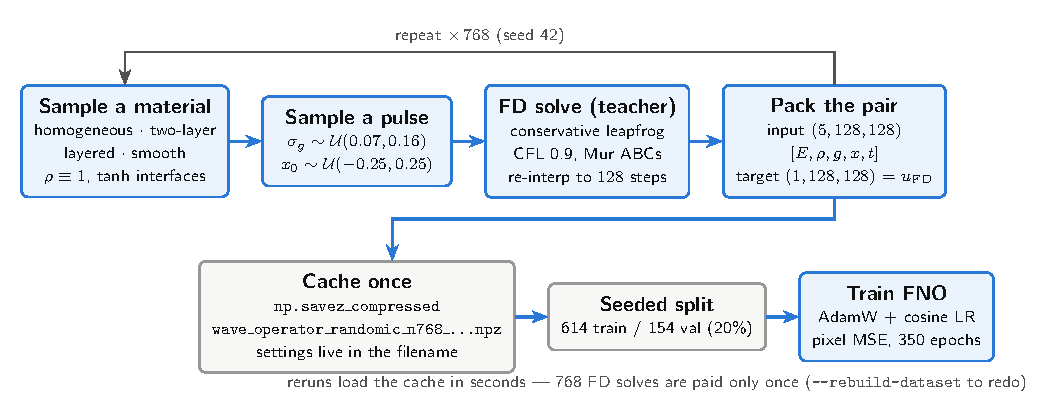
\includegraphics[width=\linewidth]{diag_data_pipeline.pdf}
  \caption{The data factory: sample a material and a pulse, let the FD solver
  produce the truth, pack the pair, cache everything once.}
  \label{fig:pipeline}
\end{figure}

\paragraph{1. Sample a random material} (\texttt{sample\_material\_profile}).
One of four families, uniformly at random; $\rho \equiv 1$ in all:
\begin{center}
\begin{tabular}{@{}lp{10.3cm}@{}}
\toprule
Family & Sampling \\
\midrule
homogeneous & constant $E \sim \mathcal{U}(0.7,\, 2.2)$ \\
two-layer   & $E_L \sim \mathcal{U}(0.7, 1.5)$, $E_R \sim \mathcal{U}(1.0, 2.5)$,
              boundary $\sim \mathcal{U}(-0.45, 0.45)$, tanh width $\sim \mathcal{U}(0.015, 0.06)$ \\
layered     & $3$--$7$ layers, values $\sim \mathcal{U}(0.7, 2.5)$; evenly spaced
              boundaries jittered by $\mathcal{N}(0, 0.04)$; chained tanh blends \\
smooth      & constant $\mathcal{U}(0.9, 1.4)$ plus 3 sine modes with amplitude
              $\mathcal{U}(-0.18, 0.18)$ and random phase; clipped to $[0.55,\, 2.5]$ \\
\bottomrule
\end{tabular}
\end{center}
This table \emph{defines the training distribution} --- the universe of
materials the FNO ever sees (Figure~\ref{fig:families}). The three canonical
materials lie inside these families by design.

\begin{figure}[htb]
  \centering
  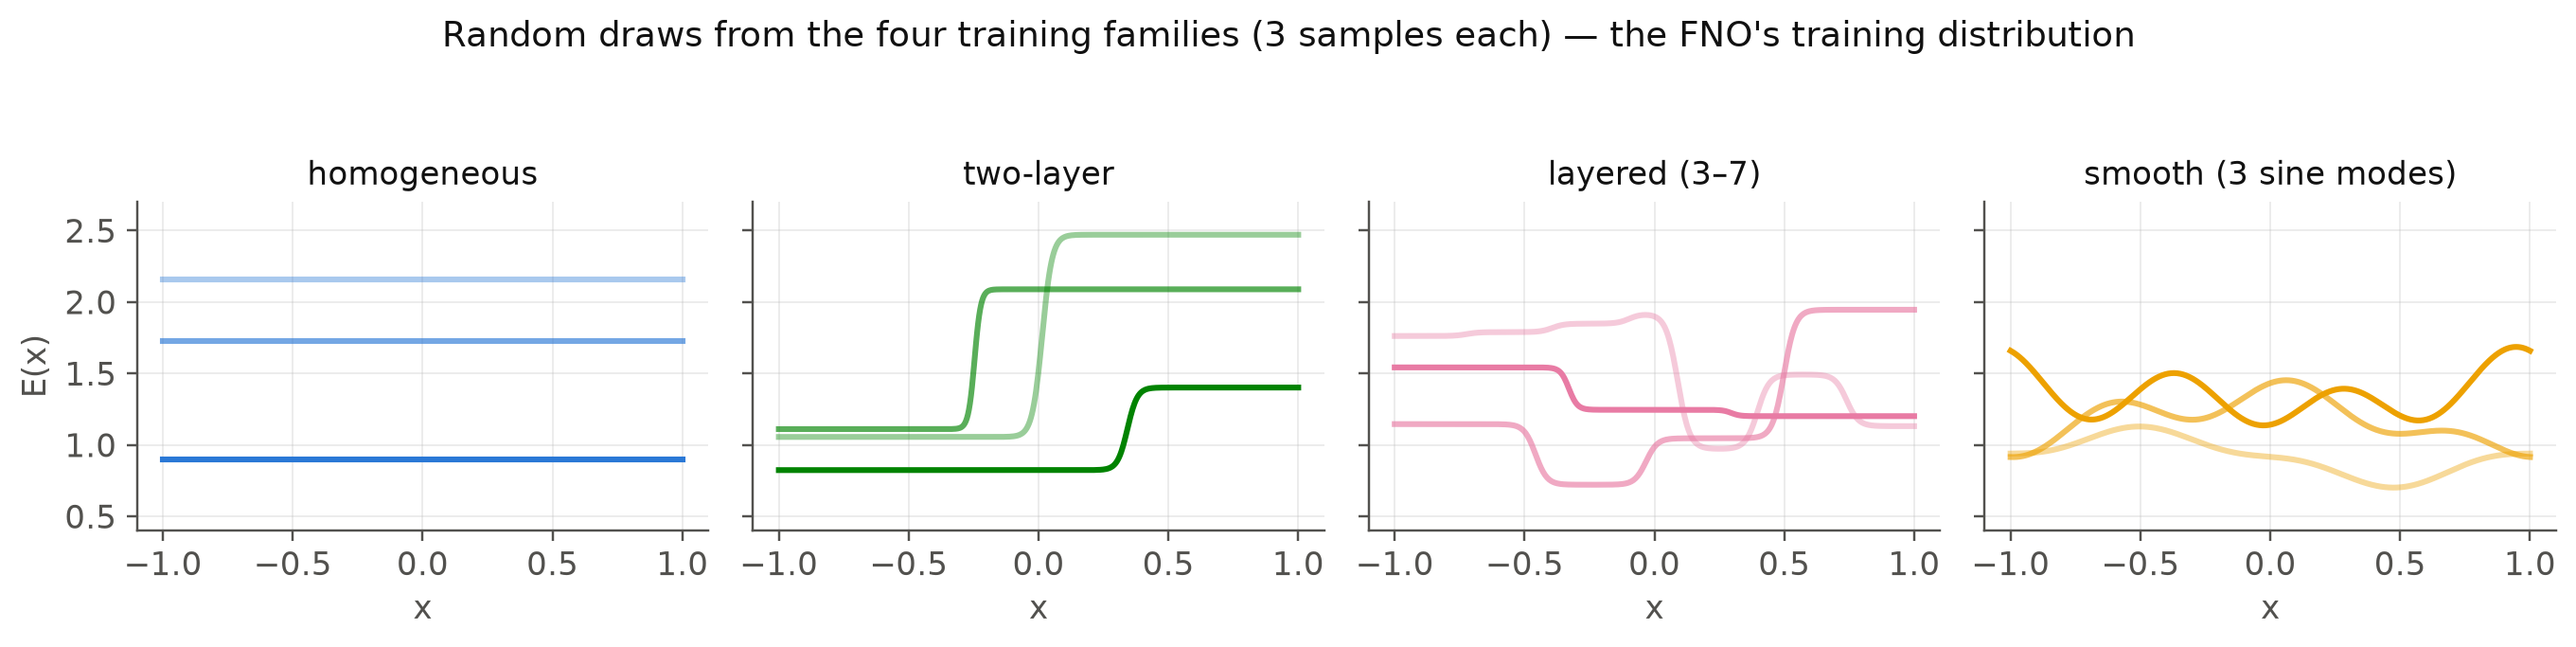
\includegraphics[width=\linewidth]{plot_random_materials.png}
  \caption{Random draws from the four material families, exactly as
  \texttt{sample\_material\_profile} produces them.}
  \label{fig:families}
\end{figure}

\paragraph{2. Sample a random pulse} (\texttt{--random-ic}):
$\sigma_g \sim \mathcal{U}(0.07, 0.16)$, $x_0 \sim \mathcal{U}(-0.25, 0.25)$.
Prevents memorization of a single source.

\paragraph{3. Solve with FD} (\texttt{solve\_case}). The sampled $E, \rho$
arrays are wrapped as interpolating functions, handed to
\texttt{solve\_wave\_1d} (CFL $0.9$), and the result is linearly re-interpolated
onto the uniform $128$-step time grid (the solver chooses its own $\Delta t$).
Solved in float64, stored as float32.

\paragraph{4. Pack question and answer} (Section~\ref{sec:encoding}), giving
per-sample tensors of shape $(5, 128, 128)$ and $(1, 128, 128)$.

\paragraph{5. Cache.} All samples are stacked and written once with
\texttt{np.savez\_compressed} to a self-describing filename,
\begin{center}
\texttt{wave\_operator\_randomic\_n768\_nx128\_nt128\_t1\_seed42.npz}
\end{center}
Every setting that changes the data (IC mode, sample count, grids, horizon,
seed) is part of the name, so a stale cache can never be loaded by mistake;
\texttt{load\_or\_generate\_dataset} loads it in seconds on reruns (or rebuilds
with \texttt{--rebuild-dataset}). A seeded shuffle then splits
$614$ train / $154$ validation (20\%).

%=====================================================================
\section{Input Encoding}
\label{sec:encoding}
%=====================================================================

\texttt{make\_input\_tensor} lays each case out as a 5-channel image over the
$(x,t)$ grid --- everything the operator is allowed to know:
\begin{equation}
  a(x,t) = \bigl[\, E(x),\; \rho(x),\; g(x),\; x,\; t \,\bigr]
  \;\longmapsto\; u(x,t).
\end{equation}
\begin{itemize}[nosep]
  \item $E$, $\rho$, $g$ depend on $x$ only; each column is broadcast
        (\texttt{np.repeat}) across all 128 time steps, so the material is
        visible at every time slice.
  \item The $x$ and $t$ \emph{coordinate channels} store each pixel's own
        position --- the standard FNO trick for positional awareness.
  \item Layout is channel-first, $(\text{batch},\, \text{channel},\, x,\, t)$
        --- the PyTorch convention expected by \texttt{Conv2d} and \texttt{rfft2}.
\end{itemize}
Batched dataset shapes: inputs $(768, 5, 128, 128)$, outputs $(768, 1, 128, 128)$.
Note the FNO predicts the \emph{entire} space--time field in one shot; it is not
autoregressive and receives no wavefield frames as input.

%=====================================================================
\section{The Spectral Layer (\texttt{SpectralConv2d})}
\label{sec:spectral}
%=====================================================================

\paragraph{Fourier background.} \texttt{rfft2}/\texttt{irfft2} translate between
``value at each grid point'' and ``how much of each spatial--temporal frequency
the field contains.'' Each frequency coefficient is a \emph{complex} number ---
amplitude and phase in one value. For \emph{real} input the negative-frequency
half of the last axis is the complex conjugate mirror of the positive half, so
\texttt{rfft2} stores only $n_t/2 + 1 = 65$ entries along $t$ (nothing is lost;
\texttt{irfft2} reconstructs the mirror). Along $x$ the full spectrum is kept,
with low positive frequencies at the start of the array and low negative
frequencies at the end.

\paragraph{The layer.} One forward pass of \texttt{SpectralConv2d}
(64 channels in/out, $m_x = m_t = 20$ modes):
\begin{enumerate}[nosep]
  \item $\hat v = \texttt{rfft2}(v)$ --- to frequency space (\texttt{norm="ortho"}).
  \item Allocate the output spectrum as \emph{zeros}: every mode above the
        cutoff is silently discarded (a learned low-pass filter).
  \item \textbf{Mix}: for each retained mode $k$, multiply the 64-vector of
        channel coefficients by that mode's own learned complex matrix
        $W(k) \in \mathbb{C}^{64\times 64}$:
        \begin{equation}
          \hat v^{\mathrm{out}}_o(k) = \sum_{i=1}^{64} W_{io}(k)\, \hat v^{\mathrm{in}}_i(k),
        \end{equation}
        implemented as \texttt{einsum("bixy,ioxy->boxy")}. Two separate weight
        tensors, \texttt{weights\_pos} and \texttt{weights\_neg}, handle the
        $+k$ and $-k$ $x$-frequency families (slices \texttt{[:mx]} and
        \texttt{[-mx:]}) --- i.e.\ right- and left-travelling wave patterns get
        independent treatment.
  \item $v^{\mathrm{out}} = \texttt{irfft2}(\hat v^{\mathrm{out}}, s{=}(n_x, n_t))$
        --- back to the grid at the exact input shape.
\end{enumerate}

\paragraph{Why complex weights.} Multiplying a frequency coefficient by a
complex number rescales the wiggle's amplitude \emph{and} slides its phase ---
and phase shift is displacement for a wave. ``Take the pulse pattern from
channel 12, move it right, weaken it 30\%, deposit it into channel 5'' is one
complex multiplication.

\paragraph{Why it is the right tool.} By the convolution theorem, pointwise
multiplication in frequency space equals a \emph{global} convolution in
physical space:
\begin{equation}
  (\mathcal{K} v)(x) = \mathcal{F}^{-1}\bigl[\, R_\theta \cdot \mathcal{F} v \,\bigr](x).
\end{equation}
One layer connects every pixel to every other --- matching the physics, where
the pulse traverses the entire domain within $t \in [0,1]$. A $3\times 3$
convolution stack would need $\sim\!60$ layers for the same reach.

\paragraph{What Mix cannot do.} Frequencies never talk to each other inside a
spectral layer (each mode is transformed independently) --- the operation is
linear. Cross-frequency interactions, which sharp interfaces require, are
created \emph{between} layers by the GELU nonlinearity in grid space. That is
the real reason the network stacks four blocks.

\begin{figure}[htb]
  \centering
  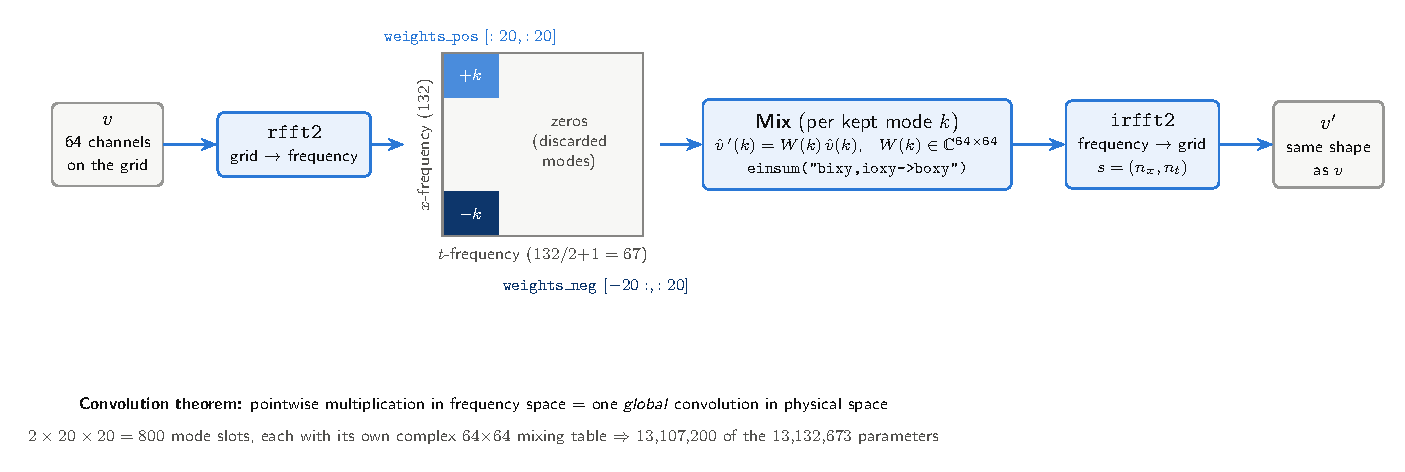
\includegraphics[width=\linewidth]{diag_spectral_conv.pdf}
  \caption{Inside \texttt{SpectralConv2d}: transform, truncate to the low-mode
  corners ($+k$ and $-k$ blocks carry \texttt{weights\_pos}/\texttt{weights\_neg}),
  mix per mode, transform back.}
  \label{fig:spectral}
\end{figure}

%=====================================================================
\section{Architecture (\texttt{FNO2d}) and Parameter Accounting}
%=====================================================================

\paragraph{One Fourier block} combines the spectral path with a local per-pixel
bypass and the nonlinearity:
\begin{equation}
  v \;\longmapsto\; \mathrm{GELU}\bigl(\, \mathrm{SpectralConv2d}(v) + W_{1\times 1}\, v \,\bigr).
\end{equation}
The $1{\times}1$ convolution bypass (a per-pixel linear map) keeps
high-frequency content alive past the mode-20 cutoff and acts as a
residual-style shortcut. The GELU is the \emph{only} nonlinearity; without it,
four stacked blocks would collapse into one linear operation
(Figure~\ref{fig:block}).

\begin{figure}[htb]
  \centering
  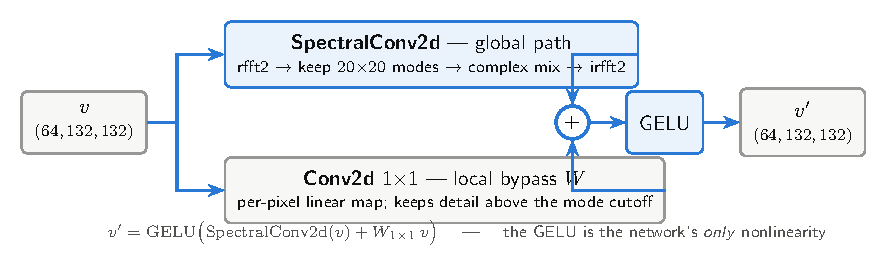
\includegraphics[width=0.9\linewidth]{diag_fourier_block.pdf}
  \caption{One Fourier block: the global spectral path and the local
  $1{\times}1$ bypass meet in a sum, followed by the GELU.}
  \label{fig:block}
\end{figure}

\paragraph{Full forward pass} (full preset: width 64, modes $20\times 20$,
4 blocks, padding 4):
\begin{center}
\texttt{5-ch input} $\to$ lift $1{\times}1$ ($5{\to}64$) $\to$ pad
$\to$ block 1 $\to$ block 2 $\to$ block 3 $\to$ block 4
$\to$ crop $\to$ project ($64{\to}128{\to}1$) $\to$ \texttt{u(x,t)}
\end{center}
The four blocks are structurally identical but share no weights --- four
independent editing stations, each with its own 800 mixing tables.
\emph{Padding:} the FFT implicitly assumes the field is periodic (wraps around
like a donut); the wavefield is not, so 4 scrap pixels are appended on the
right/bottom before the blocks and cropped after, giving wrap-around artifacts
somewhere disposable to land. Figure~\ref{fig:arch} shows the full stack with
tensor shapes and parameter counts.

\begin{figure}[htb]
  \centering
  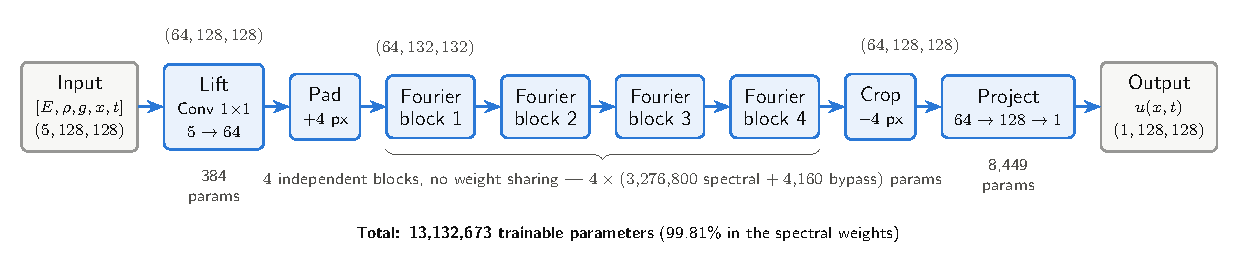
\includegraphics[width=\linewidth]{diag_fno2d_architecture.pdf}
  \caption{\texttt{FNO2d} end to end (full preset): pointwise encoder,
  four Fourier blocks, pointwise decoder.}
  \label{fig:arch}
\end{figure}

\paragraph{Parameter budget (exact).} A parameter is one trainable number.
\begin{center}
\begin{tabular}{@{}lrr@{}}
\toprule
Component & Formula & Count \\
\midrule
Spectral weights & $4 \text{ blocks} \times 2 \text{ ($\pm k$)} \times (64 \cdot 64 \cdot 20 \cdot 20)$ & 13{,}107{,}200 \\
Local $1\times1$ bypasses & $4 \times (64 \cdot 64 + 64)$ & 16{,}640 \\
Projection head & $(64 \cdot 128 + 128) + (128 \cdot 1 + 1)$ & 8{,}449 \\
Lift layer & $5 \cdot 64 + 64$ & 384 \\
\midrule
\textbf{Total} & matches \texttt{run\_summary.json} & \textbf{13{,}132{,}673} \\
\bottomrule
\end{tabular}
\end{center}
Reading the spectral formula inside-out: one $64\times 64$ mixing table per
retained mode ($4{,}096$ knobs); $20\times 20 = 400$ modes each with its own
table; $\times 2$ for the positive/negative $x$-frequency families;
$\times 4$ independent blocks. The spectral tables hold $99.81\%$ of all
parameters --- \emph{the model essentially is its frequency tables}; lift,
bypasses and projection are pointwise plumbing.

\emph{Counting caveat:} \texttt{numel} counts each complex weight once; in raw
floats the spectral part is $\approx 26$M numbers ($\approx 52$\,MB as
float32 pairs). Note also what is absent from the formula: the grid size.
Parameters attach to frequencies, not pixels --- the architectural fact behind
zero-shot evaluation at a different resolution.

%=====================================================================
\section{Training Protocol}
%=====================================================================

Training (\texttt{train\_model}) is deliberately plain supervised regression:
\begin{center}
\texttt{zero\_grad $\to$ pred = model(x) $\to$ loss = MSE(pred, $u_{\mathrm{FD}}$) $\to$ backward $\to$ step}
\end{center}
\begin{itemize}[nosep]
  \item \textbf{Loss:} pixelwise mean squared error over all $128 \times 128$
        points. No physics terms anywhere.
  \item \textbf{Optimizer:} AdamW, learning rate $8\!\times\!10^{-4} \to 10^{-5}$
        on a cosine schedule over 350 epochs; weight decay $10^{-4}$; batch size 8.
  \item \textbf{Checkpointing:} \texttt{model\_best.pt} is overwritten only when
        validation MSE improves and is \emph{reloaded at the end} --- the
        delivered model is the best generalizer, not the last epoch.
        \texttt{model\_latest.pt} (with optimizer and scheduler state) is
        written every 10 epochs so \texttt{--resume} survives Kaggle session kills.
  \item \textbf{Mixed precision:} off by default (cuFFT under autocast can be
        unstable); \texttt{torch.compile} optional.
\end{itemize}

\paragraph{What is absent --- on purpose.} No PDE residual, no collocation
points, no causal weighting, no GradNorm, no RBA, no L-BFGS phase, no ansatz.
The PINN machinery exists because the physics loss is hard to optimize;
supervision with FD labels removes the difficulty --- at the price of a dataset
(768 FD solves paid up front).

\paragraph{Kaggle presets} (\texttt{kaggle/run\_fno\_t4.py}), one T4 GPU:
\begin{center}
\begin{tabular}{@{}lrrrrrrr@{}}
\toprule
Preset & Samples & Train grid & Eval grid & Epochs & Width & Modes & Params \\
\midrule
smoke  & 32  & $64^2$  & $96^2$  & 10  & 16 & $8\times8$   & $\approx$0.1M \\
medium & 256 & $128^2$ & $192^2$ & 150 & 48 & $16\times16$ & $\approx$4.7M \\
full   & 768 & $128^2$ & $256^2$ & 350 & 64 & $20\times20$ & 13.1M \\
\bottomrule
\end{tabular}
\end{center}

%=====================================================================
\section{The Control Experiment (\texttt{ConvBaseline2d})}
%=====================================================================

A plain CNN with the identical 5-in/1-out tensor interface: six $3\times 3$
convolutions with GELU (\texttt{--compare-cnn} trains both models). Each
$3\times 3$ layer grows the receptive field by 2 pixels, so after 6 layers each
output pixel sees only $\approx 13$ pixels --- while the wave physically
traverses all 128. The CNN \emph{cannot} see the far side of the domain.
If the FNO wins, the credit demonstrably belongs to global spectral mixing,
not to generic deep-learning capacity.

%=====================================================================
\section{Evaluation Protocol and Results}
%=====================================================================

\paragraph{Metric.} Per-sample relative $L_2$ error, in percent:
\begin{equation}
  \varepsilon = 100 \cdot \frac{\lVert u_{\mathrm{pred}} - u_{\mathrm{FD}} \rVert_2}
                           {\lVert u_{\mathrm{FD}} \rVert_2}.
\end{equation}

\paragraph{Two exams.}
\begin{enumerate}[nosep]
  \item \textbf{Validation} --- 154 held-out random cases at the training
        resolution ($128^2$): in-distribution generalization.
  \item \textbf{Canonical materials} (\texttt{evaluate\_reference\_materials})
        --- the three official materials with the fixed pulse
        ($\sigma_g{=}0.1$, $x_0{=}0$), evaluated at $256^2$: \emph{twice} the
        training resolution, zero-shot (parameters live on frequencies, so the
        same weights run on any grid). FD truth is regenerated on the finer grid.
\end{enumerate}

\paragraph{Results (full preset, \texttt{fno\_t4\_full/run\_summary.json}).}
\begin{center}
\begin{tabular}{@{}lr@{}}
\toprule
Benchmark & Rel.\ $L_2$ \\
\midrule
Validation ($128^2$, in-distribution) & $3.21\%$ \\
Homogeneous ($256^2$)  & $28.35\%$ \\
TwoLayer ($256^2$)     & $31.18\%$ \\
MultiLayer ($256^2$)   & $36.44\%$ \\
\bottomrule
\end{tabular}
\end{center}
Across presets, validation error falls $94.8\% \to 7.4\% \to 3.2\%$
(smoke $\to$ medium $\to$ full); train MSE reaches $1.0\times 10^{-6}$ with
validation MSE plateauing at $1.3\times 10^{-4}$ --- converged, with a widening
train/val gap (Figure~\ref{fig:history}).

\begin{figure}[htb]
  \centering
  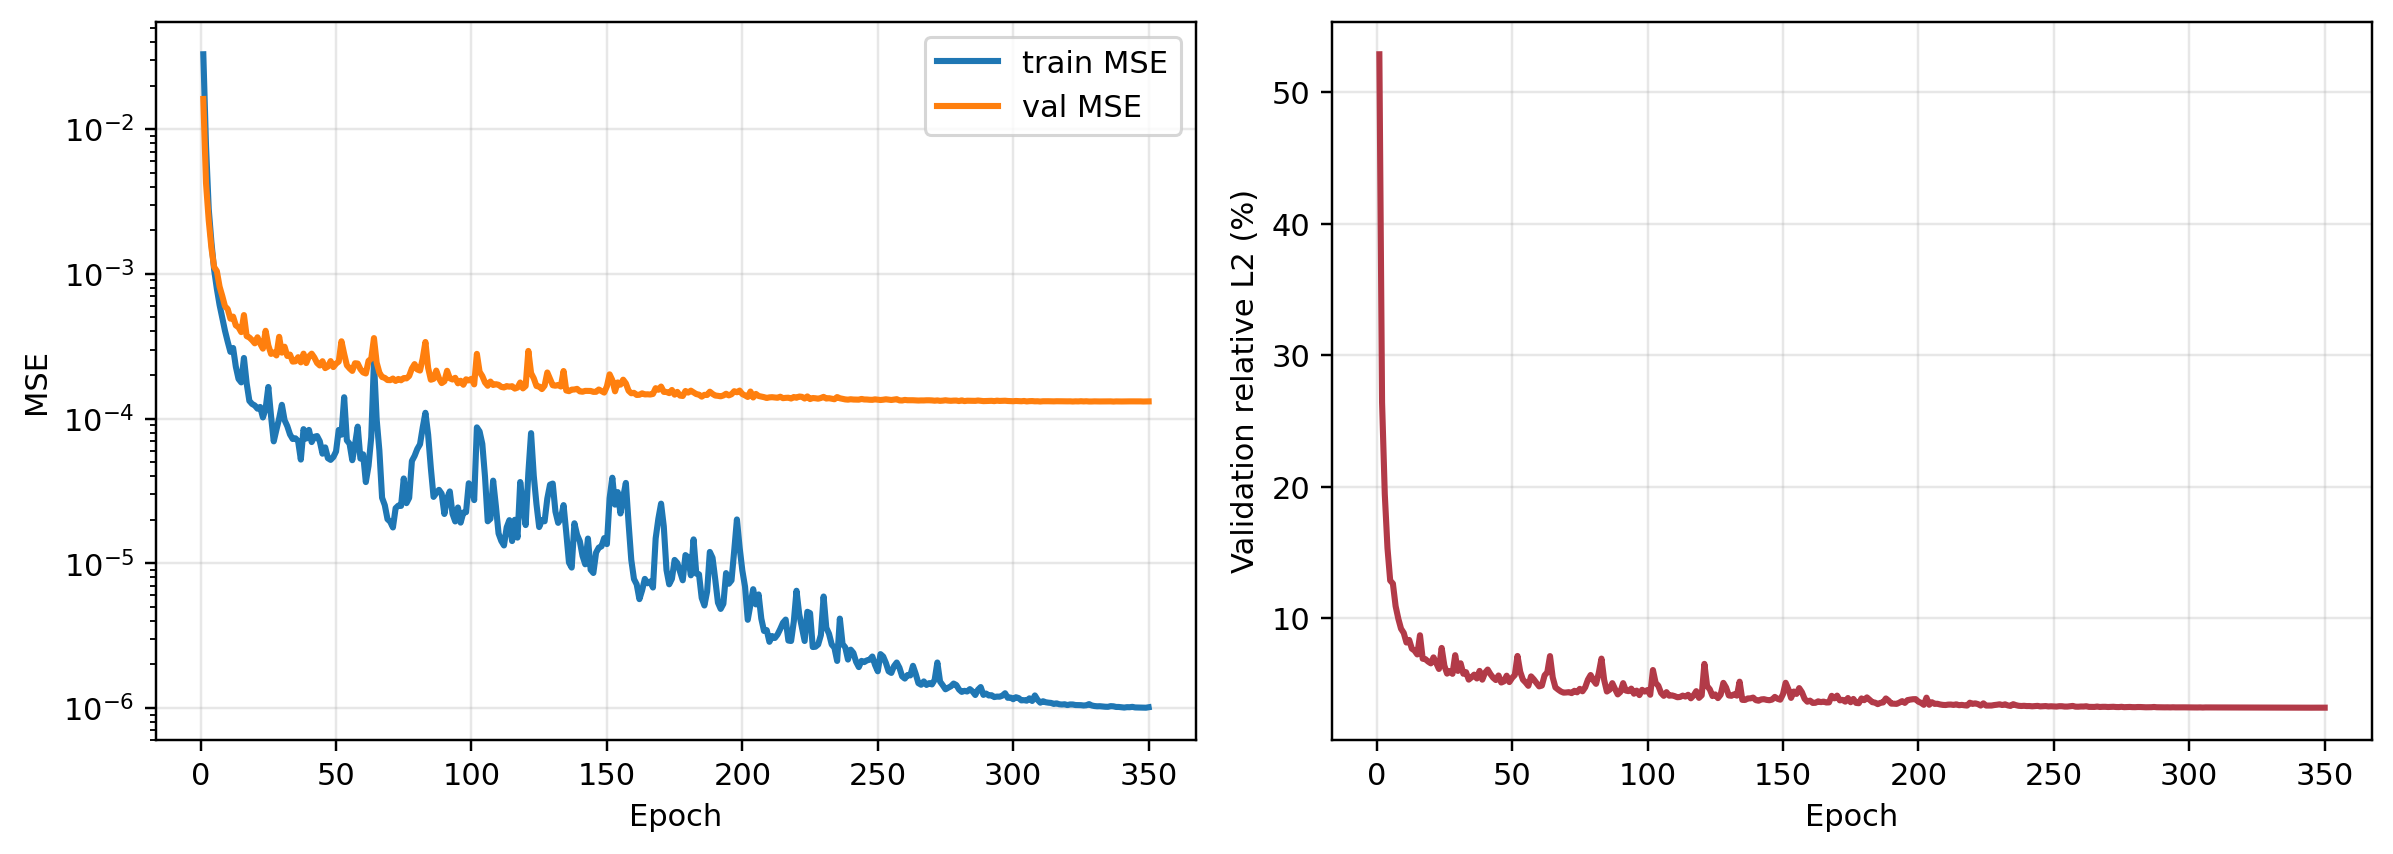
\includegraphics[width=\linewidth]{history.png}
  \caption{Training history of the full T4 run. Left: train/val MSE (log scale)
  --- the widening gap shows mild overfitting after convergence. Right:
  validation relative $L_2$ settling at $3.2\%$.}
  \label{fig:history}
\end{figure}

\begin{figure}[p]
  \centering
  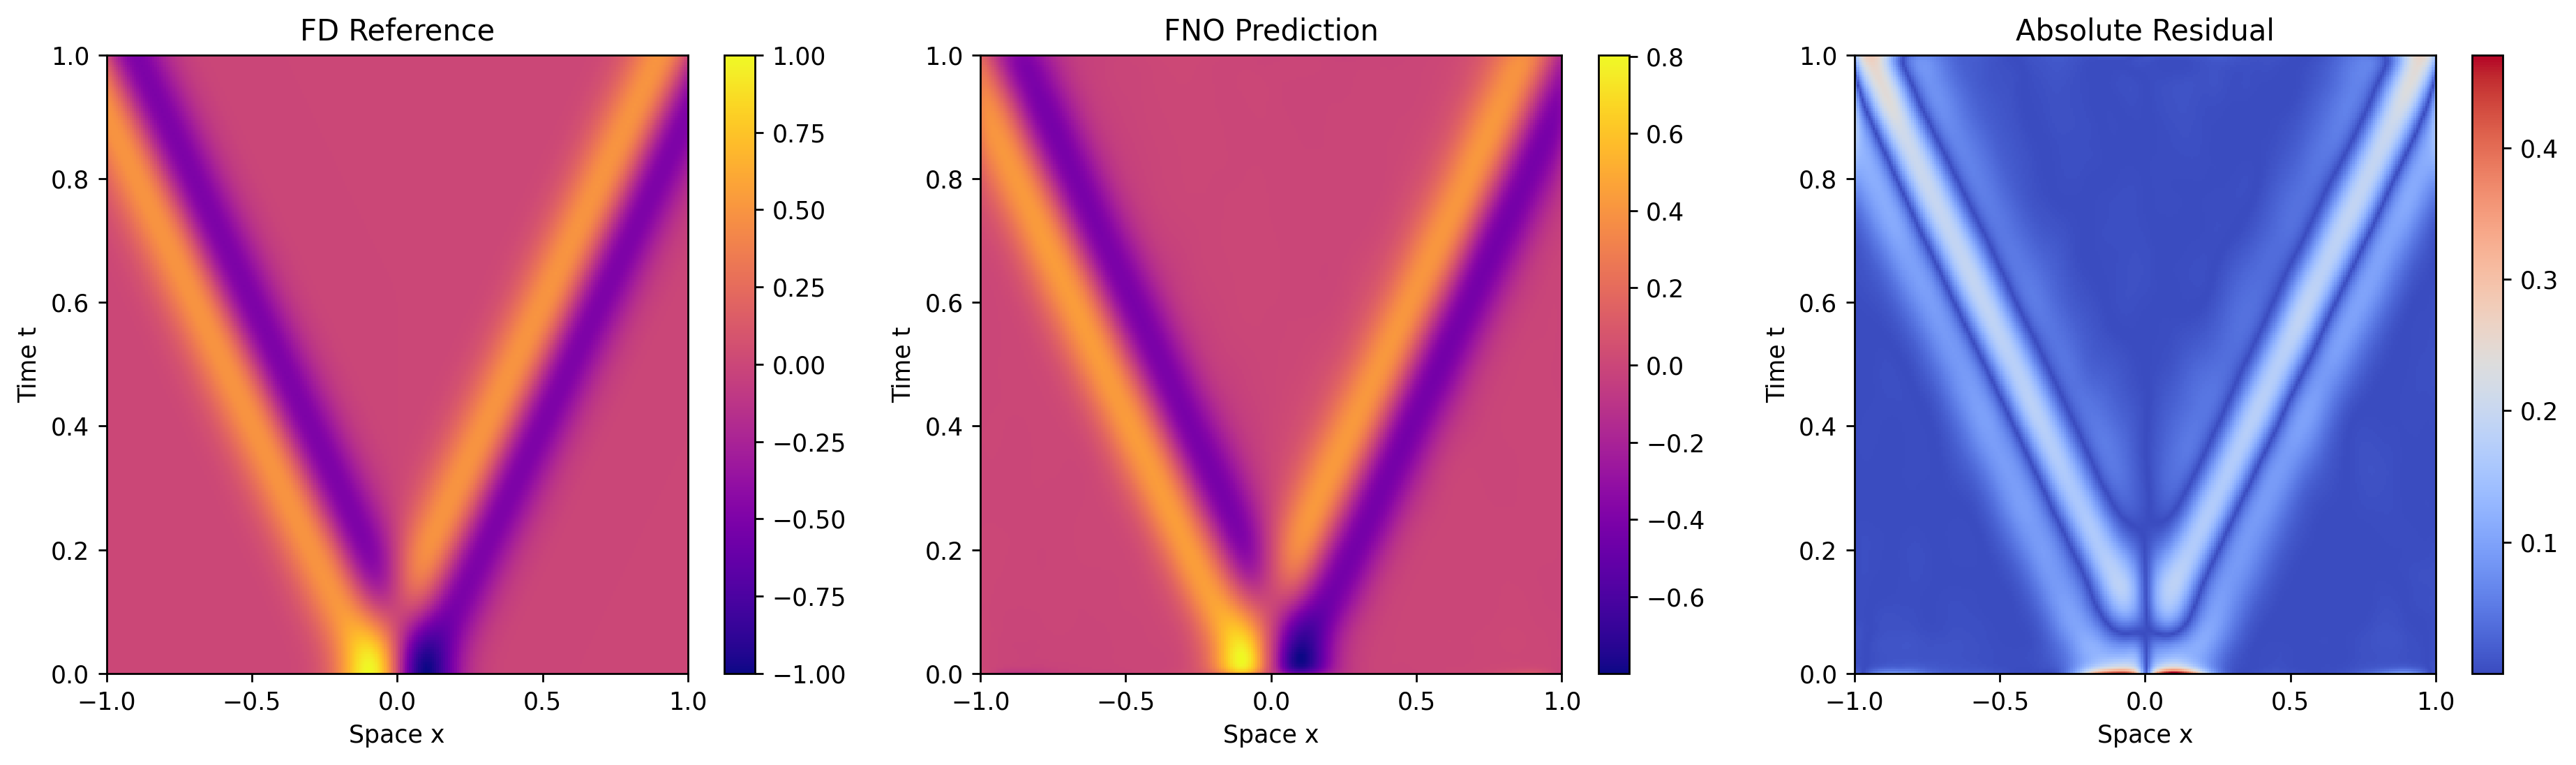
\includegraphics[width=\linewidth]{Homogeneous_solution_comparison.png}\\[4pt]
  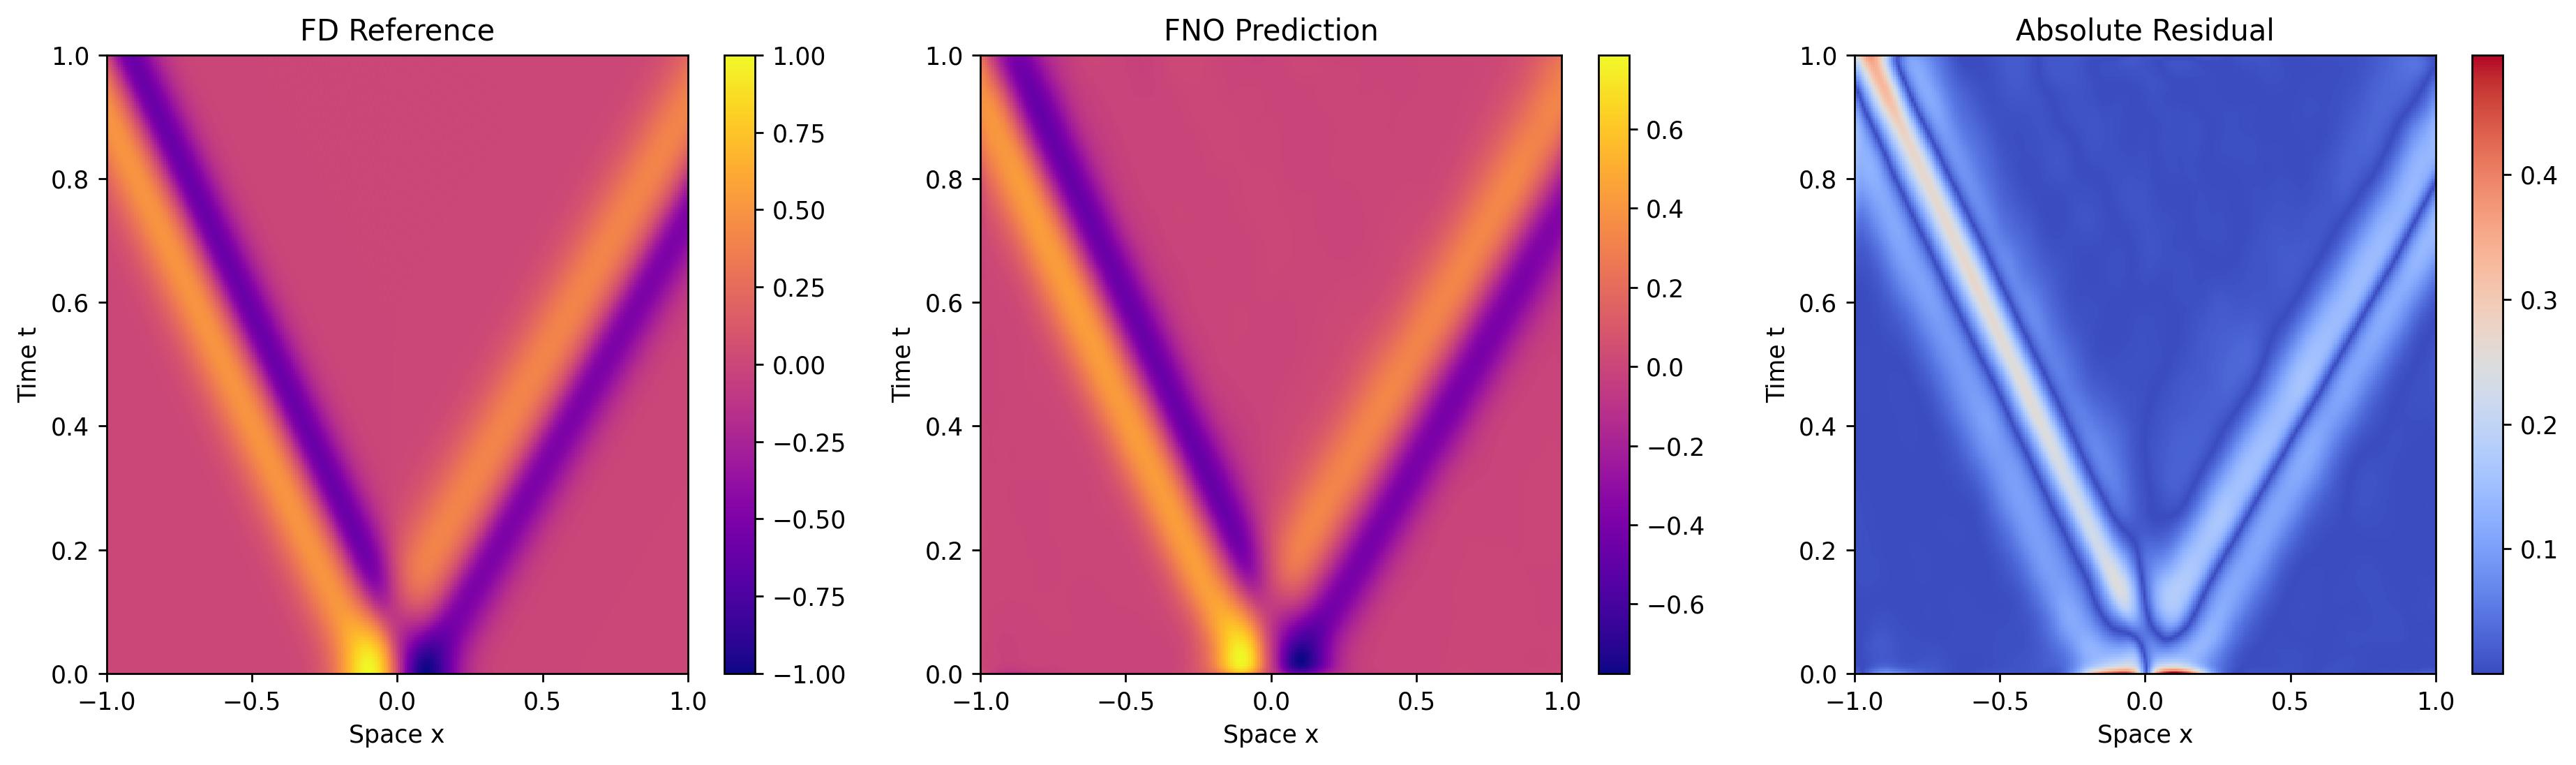
\includegraphics[width=\linewidth]{TwoLayer_solution_comparison.png}\\[4pt]
  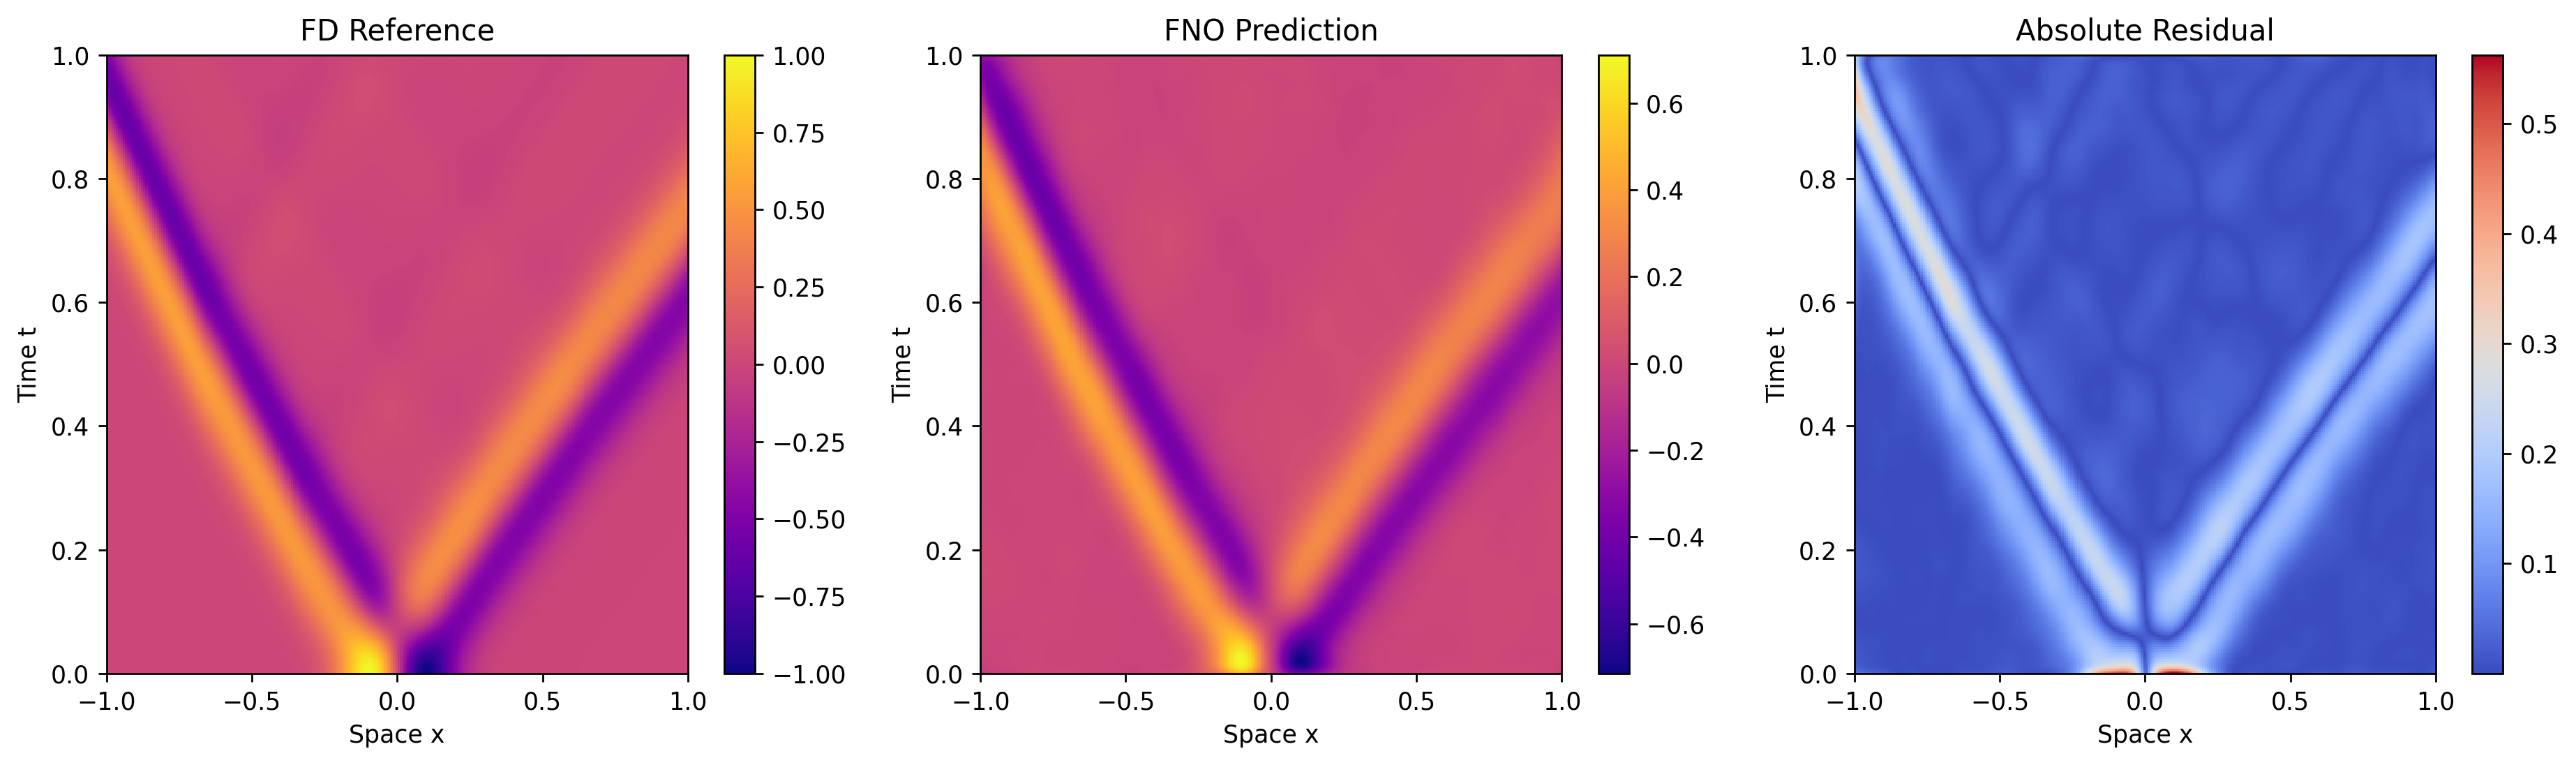
\includegraphics[width=\linewidth]{MultiLayer_solution_comparison.png}
  \caption{The canonical-material exam at $256\times256$ (top to bottom:
  Homogeneous, TwoLayer, MultiLayer). Each row: FD reference $|$ FNO prediction
  $|$ absolute residual. The wave geometry and amplitudes are tracked well; the
  residual concentrates on the wavefronts and the $t=0$ cusp --- a
  phase/sharpness offset rather than a geometry error --- and grows with
  material complexity (28.4\%, 31.2\%, 36.4\%).}
  \label{fig:comparisons}
\end{figure}

\paragraph{The open question.} The $3\% \to 30\%$ gap conflates two changes
made simultaneously: (i) zero-shot super-resolution ($128 \to 256$; the FD
reference itself also sharpens at higher resolution), and (ii) the switch from
random draws to the fixed canonical cases. The clean diagnostic --- re-running
the canonical benchmark at the training resolution
(\texttt{--eval-nx 128 --eval-nt 128}) --- decomposes the error into
resolution-transfer vs.\ everything else, and is the first item on the
next-runs list. Until then, calling the 36\% ``out-of-distribution'' is
imprecise: the canonical materials arguably lie \emph{inside} the sampled
families; what mainly changed is the grid.

%=====================================================================
\section{The Second FNO: Ansatz-Conditioned (\texttt{final/ML})}
%=====================================================================

The repository contains a second, deliberately different FNO
(\texttt{final/ML/src/models.py}: \texttt{FNO1d}, \texttt{FNOWrapper};
trainer \texttt{training\_code\_fno.py}):

\begin{itemize}[nosep]
  \item \textbf{1D, per time slice.} A 1D spectral operator over $x$ only
        (32 modes, width 64); the query time $t$ enters as an input channel:
        $[x, E(x), g(x), t] \mapsto$ one spatial slice.
  \item \textbf{Predicts the ansatz NN term, not $u$.} The raw output is plugged
        into the blank of the hard-constraint template \eqref{eq:ansatz}
        (\texttt{pred = apply\_ansatz(nn\_out, ...)}) \emph{before} the MSE
        against FD --- so the initial condition is exact by construction and the
        model inherits the PINN arm's guarantee.
  \item \textbf{Per-material operator over the pulse width.} Trained on a bank
        of 32 FD solves of \emph{one} material with
        $\sigma_g \sim \mathcal{U}(0.05, 0.2)$ (the canonical $\sigma_g = 0.1$
        guaranteed in the bank); an operator over initial conditions, not materials.
  \item \textbf{Purpose:} it speaks the pointwise \texttt{model(x,t)} interface
        of \texttt{benchmark\_v2.py}, so the FNO can sit in the same comparison
        table as the seven PINN architectures, apples-to-apples.
\end{itemize}

\paragraph{Comparison of the two baselines.}
\begin{center}
\begin{tabular}{@{}p{3.4cm}p{5.0cm}p{5.2cm}@{}}
\toprule
 & \texttt{wave/} (grid-to-grid) & \texttt{final/ML} (ansatz-conditioned) \\
\midrule
Mapping & $[E,\rho,g,x,t] \to u(x,t)$, whole field at once & $[x,E,g,t] \to$ ansatz NN term, slice by slice \\
Generalizes over & materials and pulses & pulse width, one material \\
IC handling & learned from data & exact via ansatz \\
Reported accuracy & 3.2\% val; 28--36\% canonical @ $256^2$ & 2.53\% best mean $L_2$, exp1 (Homogeneous) \\
Status & smoke/medium/full converged & exp1 only; exp2/3 not yet run \\
\bottomrule
\end{tabular}
\end{center}

\begin{figure}[htb]
  \centering
  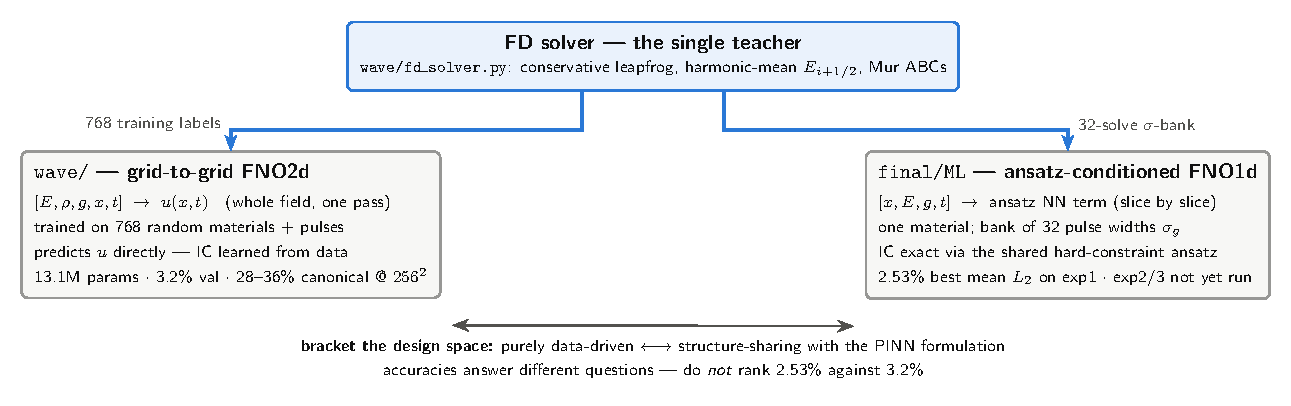
\includegraphics[width=\linewidth]{diag_two_baselines.pdf}
  \caption{One teacher, two complementary FNO baselines.}
  \label{fig:twobaselines}
\end{figure}

\textbf{Comparability caveat.} The 2.53\% and 3.2\% numbers answer different
questions and must not be ranked against each other: exp1 is the easiest
material, evaluated at the canonical pulse that was deliberately included in
its training bank, while the \texttt{wave/} numbers span random materials and
a doubled evaluation grid. Likewise, ``physics-constrained'' overstates the
second model: the ansatz enforces only the initial condition exactly; there is
still no PDE term in either loss. The honest framing: the two FNOs bracket the
design space from purely data-driven (grid-to-grid) to structure-sharing with
the PINN formulation (IC-hard-constrained).

%=====================================================================
\section{Quick-Reference Numbers}
%=====================================================================

\begin{center}
\begin{tabular}{@{}lp{8.6cm}@{}}
\toprule
768 / 614 / 154 & samples total / train / validation (full preset) \\
$(768,5,128,128)$ & input tensor: samples $\times$ channels $\times$ $x$ $\times$ $t$ \\
5 channels & $E(x)$, $\rho(x)$, $g(x)$, $x$-mesh, $t$-mesh \\
$20 \times 20$ ($\times 2$) & retained modes per axis (positive and negative $x$-families) \\
13{,}132{,}673 & trainable parameters; 99.81\% spectral; $\approx 26$M raw floats \\
$8\!\times\!10^{-4} \to 10^{-5}$ & AdamW cosine learning-rate schedule, 350 epochs, batch 8 \\
3.21\% & validation relative $L_2$ (in-distribution, $128^2$) \\
28.35 / 31.18 / 36.44\% & Homogeneous / TwoLayer / MultiLayer at $256^2$, zero-shot \\
2.53\% & \texttt{final/ML} ansatz-conditioned FNO, exp1 canonical window \\
$\mathrm{CFL} = 0.9$ & FD stability safety factor; harmonic-mean $E_{i+1/2}$; Mur ABCs \\
\bottomrule
\end{tabular}
\end{center}

%=====================================================================
\section*{Key References}
%=====================================================================
\begin{itemize}[nosep]
  \item Li, Kovachki, Azizzadenesheli et al., \emph{Fourier Neural Operator for
        Parametric Partial Differential Equations}, arXiv:2010.08895 (2020).
  \item Wang, Sankaran, Perdikaris, \emph{Respecting causality is all you need
        for training physics-informed neural networks}, arXiv:2203.07404 (2022).
  \item Wang et al., \emph{An Expert's Guide to Training Physics-Informed
        Neural Networks}, arXiv:2308.08468 (2023).
  \item Anagnostopoulos et al., \emph{Residual-based attention for PINNs},
        arXiv:2307.00379 (2023).
  \item Vyas et al., \emph{SOAP: Improving and stabilizing Shampoo},
        arXiv:2409.11321 / 2502.00604.
  \item Repository: \texttt{wave/run\_fno\_baseline.py},
        \texttt{src/operator\_baselines.py}, \texttt{wave/fd\_solver.py},
        \texttt{wave/materials.py}, \texttt{wave/problem\_data.py},
        \texttt{final/ML/training\_code\_fno.py}; curated reading order in
        \texttt{papers/FNO\_reading\_order/}.
\end{itemize}

\end{document}
